\section{Introduction}
\label{sec:intro}

Fine-tuning a pretrained language model on a narrow domain is the standard way to specialise it. It also erodes the model's general abilities, a problem known as catastrophic forgetting~\citep{mccloskey1989catastrophic,luo2023empirical}. Practitioners who want to stop training before too much is lost must evaluate general benchmarks at every checkpoint, which is slow and needs labelled data. A cheaper option is to watch the model's \emph{representation geometry} on a fixed set of probe texts. If a pretrained model's neighbourhood structure collapses before or while it forgets, a label-free geometric monitor could replace part of the benchmark suite.

{\bf How fast does fine-tuning destroy pretraining geometry?} Prior work shows that fine-tuning changes representations~\citep{merchant2020happens}, that contextual embeddings are anisotropic~\citep{ethayarajh2019contextual,mu2018allbutthetop}, and that forgetting grows with the amount of fine-tuning and shrinks with model size~\citep{kalajdzievski2024scaling,biderman2024lora}. These studies mostly report end states or global similarity scores. They leave open three practical questions. First, how many steps does it take for local neighbourhood structure to fall apart, and does this depend on scale? Second, does a geometric quantity cross a fixed threshold when forgetting begins? Third, does the fine-tuning domain matter, and is lexical closeness to pretraining data a good predictor?

We turn these questions into four specific hypotheses. \textbf{H1}: \pres of general-text probes falls below 50\% within 500 steps for sub-1B models but only after 2,000 steps for 7B models. \textbf{H2}: isotropy decreases monotonically. \textbf{H3}: general-knowledge accuracy starts to decline once preservation drops below 60\%. \textbf{H4}: medical fine-tuning preserves more structure than code fine-tuning because medical text shares more vocabulary with pretraining data.

We test them with a step-resolved study (\figref{fig:trajectories}). We fine-tune five base models (\pythiaS, \pythiaM, \qwenS, \qwenM, \qwenL) on synthetic clinical notes, Python code, and a \wikitext control, and evaluate 17 checkpoints between step 0 and step 3,000. At each checkpoint we measure kNN neighbourhood preservation, CKA, and three isotropy measures on 1,000 held-out probes. We also measure general knowledge on 1,070 \mmlu and \arce items with item-level paired tests, and perplexity on general and in-domain text. Learning-rate and full fine-tuning ablations separate the effect of model size from the effect of update size.

{\bf None of the four hypotheses holds as stated.} Within each model family, larger models do keep more of their geometry at matched steps: after 500 medical steps, preservation is 0.42, 0.74, 0.79, 0.82, and 0.85 for the 160M, 410M, 0.5B, 1.5B, and 3B models. But \qwenS never falls below 0.71 under the standard recipe, while the same model reaches 0.22 when the learning rate is 1e-3. All seven runs that ended below 0.5 had rising held-out in-domain loss. No run became monotonically less isotropic on any of three measures. In Qwen models, significant benchmark forgetting begins at preservation 0.77--0.90, far above 0.6. Medical fine-tuning preserves more general-text geometry than code fine-tuning at only 17\% of matched checkpoints. This happens even though clinical notes are lexically much closer to general text (unigram JSD 0.45 \versus 0.63 bits). Preservation is still useful: it tracks damage to general-text language modelling with Spearman $\rho=-0.90$, and a sharp early drop reliably flags unstable training.

Our contributions are:
\begin{itemize}[leftmargin=*,itemsep=0pt,topsep=0pt]
    \item We conduct a step-resolved study of embedding drift across 22 fine-tuning runs, five model sizes, two families, three domains, and two training methods, with item-level forgetting tests at every checkpoint.
    \item We show that the speed of neighbourhood collapse depends more on the learning rate and on training stability than on model size, and that collapse below 50\% happens only in runs whose in-domain loss rises.
    \item We find that global isotropy is a weak, non-monotone drift signal, and that no fixed preservation threshold marks the start of benchmark forgetting.
    \item We find that vocabulary overlap does not predict geometric preservation: code fine-tuning preserves more general-text geometry than medical fine-tuning, and we identify the confound (how much there is to learn) that a follow-up design must remove.
\end{itemize}

\Secref{sec:related} reviews related work. \Secref{sec:method} describes the models, data, and metrics. \Secref{sec:results} tests each hypothesis. \Secref{sec:discussion} discusses implications and limitations, and \secref{sec:conclusion} concludes.

\begin{figure}[t]
    \centering
    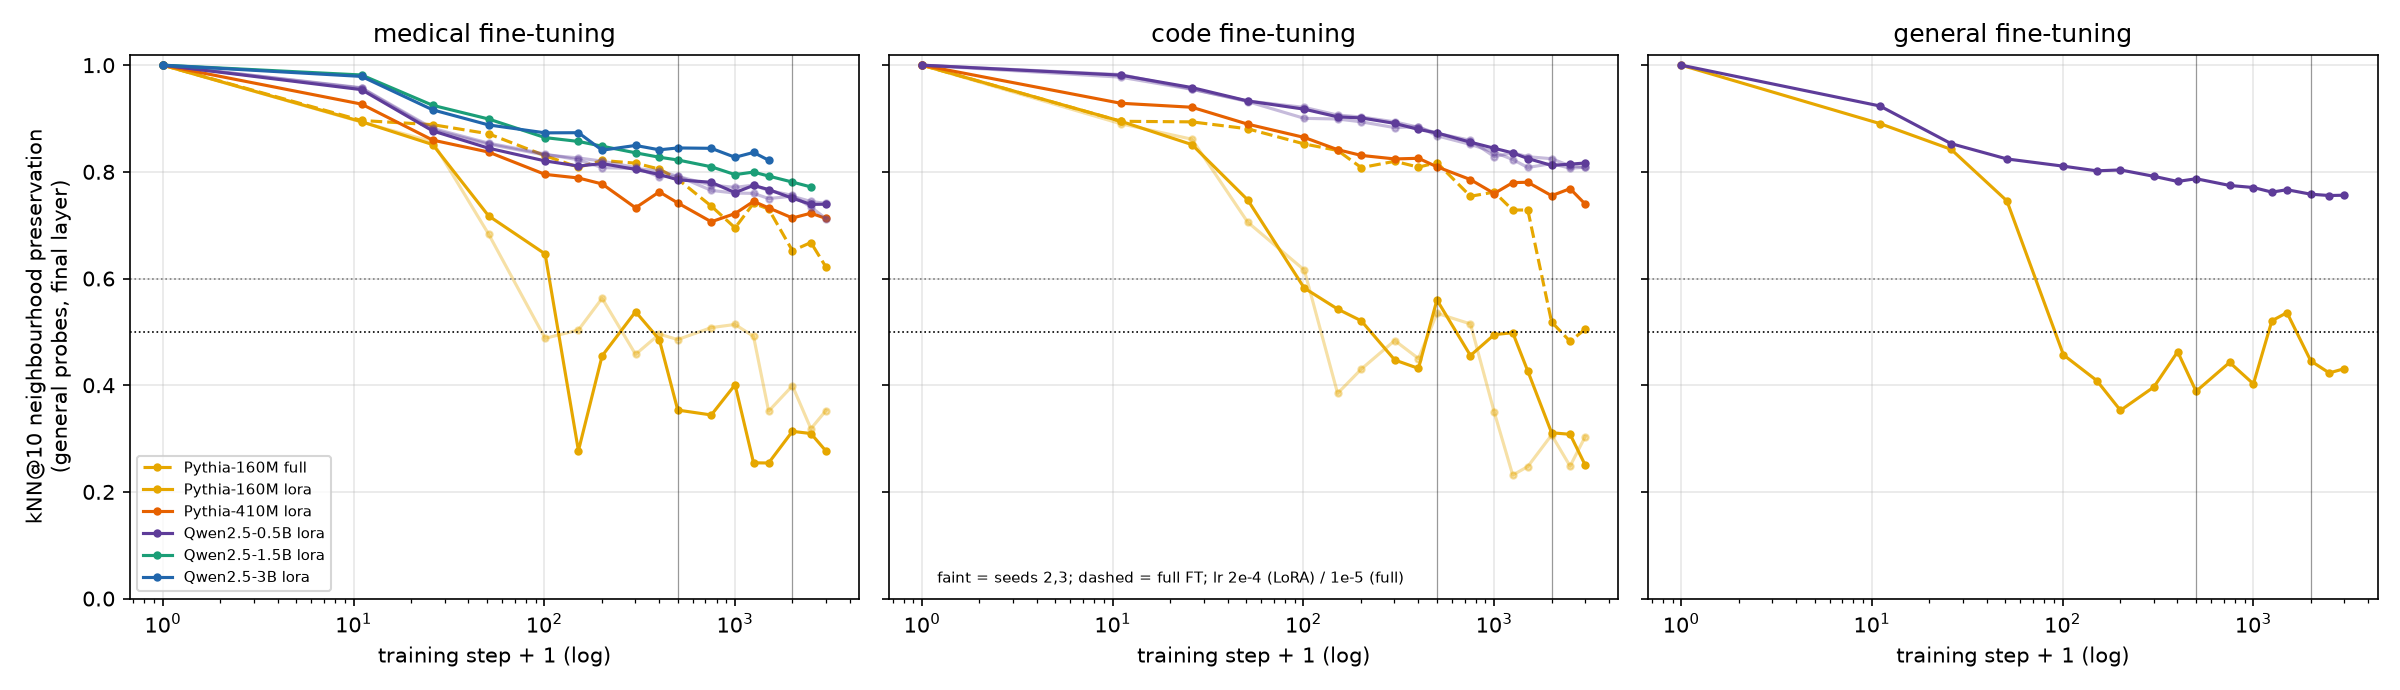
\includegraphics[width=0.98\linewidth]{figures/fig1_preservation_trajectories.png}
    \caption{\pres of 1,000 general-text probes (final layer) against training step for medical, code, and general fine-tuning. Faint lines are additional seeds; dashed lines are full fine-tuning of \pythiaS. Most of the loss happens in the first $\sim$100 steps. Larger Qwen models drift less, but only \pythiaS under LoRA falls below 0.5 (dotted line) with the standard recipe, and all those runs diverged in in-domain loss.}
    \label{fig:trajectories}
\end{figure}
